\documentclass{article}
%\usepackage{fullpage}
\usepackage{fancyhdr}
\usepackage[english,francais]{babel}
\usepackage[T1]{fontenc}
\usepackage[utf8]{inputenc}
\usepackage[pdftex]{graphicx}
\usepackage{subfig}

%\renewcommand{\baselinestretch}{2}
\author{Brieuc \textsc{Daniel}, Océane \textsc{Lasserre}, Danchi \textsc{Li}, \\ Florent \textsc{Guiotte}, Frédéric \textsc{Becker}}
\title{Moteur de recherche d'images \\ \Large{Compte rendu de résultats}}
\pagestyle{fancy}

\begin{document}
\maketitle
\tableofcontents

\section{Introduction}

Le but de ce projet est de développer un moteur de recherche dans une base de données. 

Le projet se divise en deux parties, une <<Offline>> qui extrait et indexe des descripteurs sur une base de données
d'images. Une autre dite <<Online>> extrait ce même type de descripteur sur une image requête, et cherche des
correspondances avec la base des descripteurs générée en <<Offline>>. La correspondance se fait à l'aide d'un 
algorithme de vote. Les meilleurs résultats sont alors affichés selon leur pertinence. 

Pour ce projet nous utiliserons deux types de descripteurs distincts.
Le descripteur {\em Speeded Up Robust
Features (SURF)} et le descripteur {\em Scale-invariant feature transform (SIFT)}.

\section{Tests et résultats}
\subsection{Tests avec différents descripteurs}

Sur une même base de données, nous avons testé l'algorithme avec deux descripteurs différents.

\subsubsection{SURF}

La fonction SURF donne les résultats de la figure \ref{surf}.

\begin{figure}[!ht]%htp]
  \centering
  \subfloat[SURF - knn]{\label{surf:knn}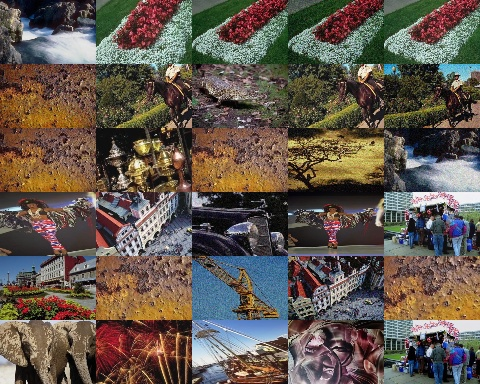
\includegraphics[width=0.49\textwidth]{img/KMeansIndex/knn/corel_0000000303_512_COREL_SURF.jpg}}
  \hspace{0.01\textwidth}
  \subfloat[SURF - Spheric]{\label{surf:spheric}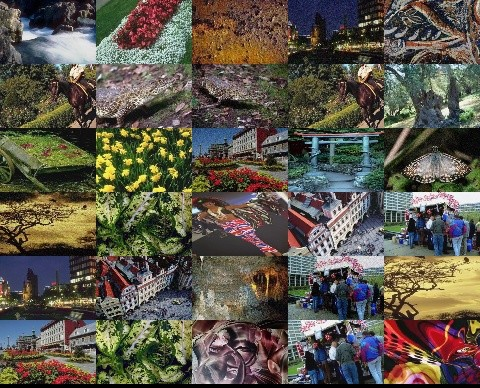
\includegraphics[width=0.49\textwidth]{img/KMeansIndex/radius/corel_0000000303_512_COREL_SURF.jpg}}
  \caption{Résultats avec SURF via une recherche knn et sphérique.}
  \label{surf}
\end{figure}

L'image en haut à gauche de chaque figure correspond à l'image requête retrouvée. Les images suivantes sont
classées de la plus pertinente à la plus eloignée (de gauche à droite).
On observe que les résultats sont éloignés de l'image requête. 

L'image requête est bien retrouvée mais les autres images obtenues ne sont pas pertinentes et les images les
plus proches <<instinctivement>> ne sont pas retrouvées. 
Le type de recherche (knn ou sphérique) a une influence importante sur les résultats mais ne semble pas les rapprocher de l'image requête. 

\subsubsection{SIFT}

La fonction SIFT donne les résultats de la figure \ref{sift} (sur les mêmes images requêtes que précédemment).

\begin{figure}[!ht]%htp]
  \centering
  \subfloat[SIFT - knn]{\label{sift:knn}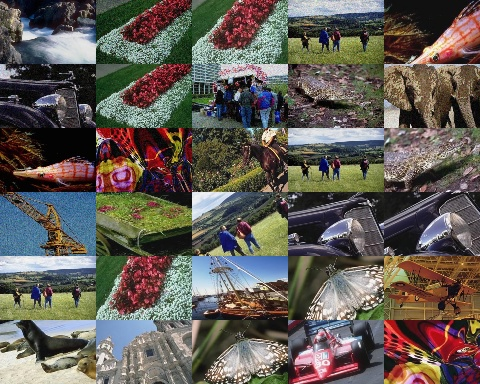
\includegraphics[width=0.49\textwidth]{img/KMeansIndex/knn/corel_0000000303_512_COREL_SIFT.jpg}}
  \hspace{0.01\textwidth}
  \subfloat[SIFT - Spheric]{\label{sift:spheric}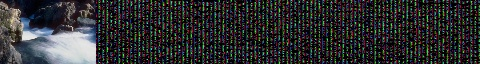
\includegraphics[width=0.49\textwidth]{img/KMeansIndex/radius/corel_0000000303_512_COREL_SIFT.jpg}}
  \caption{Résultats avec SIFT via une recherche en knn et sphérique.}
  \label{sift}
\end{figure}

L'image en haut à gauche de chaque figure correspond à l'image requête retrouvée. Les images suivantes sont
classées de la plus pertinente à la plus eloignée (de gauche à droite).

La pertinence des résultats ici est la même que pour les descripteurs SURF. En revanche dans ce cas précis, cela vient du fait que pour une recherche sphérique,
seule l'image requête est trouvée. Les autres sont trop éloignées pour être conservées. Le nombre de <<vrais
positifs>> n'est pas amélioré mais cela diminue 
le nombre de <<faux positifs>>. Selon le type de recherche, cela peut être, ou non, un avantage.


\subsection{Tests sur différentes bases de données}

Avec le même descripteur, nous avons testé l'algorithme sur la base de donnée {\em NISTER}. Cette base
d'image propose des échantillons de transformation\footnote{Rotations, translations, bruitage\ldots} sur quelques images.
Les résultats sont visibles figure \ref{db}. Les résultats semblent plus pertinents sur cette base de données,
surtout avec les descripteurs SIFT (cf. figure \ref{db:sift}).

\begin{figure}[!ht]%htp]
  \centering
  \subfloat[SIFT]{\label{db:sift}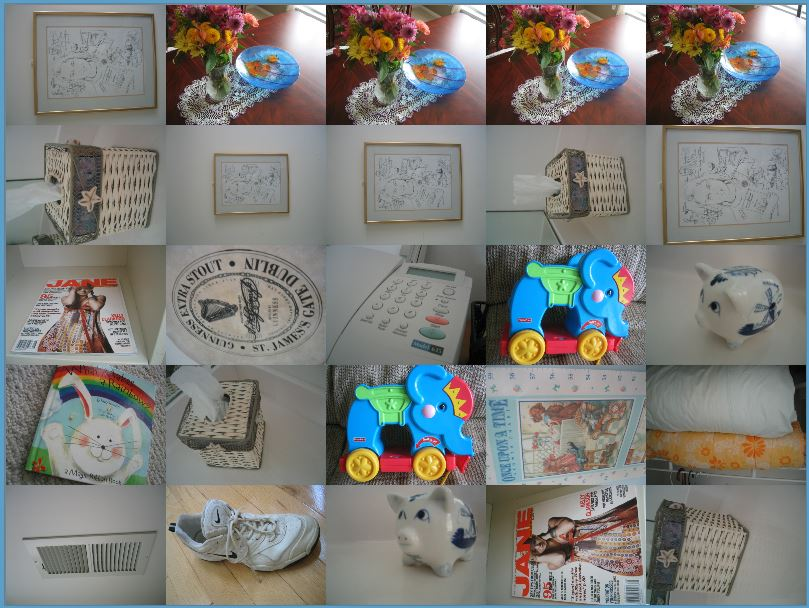
\includegraphics[width=0.49\textwidth]{img/sift_knn=25_linear.JPG}}
  \hspace{0.01\textwidth}
  \subfloat[SURF]{\label{db:surf}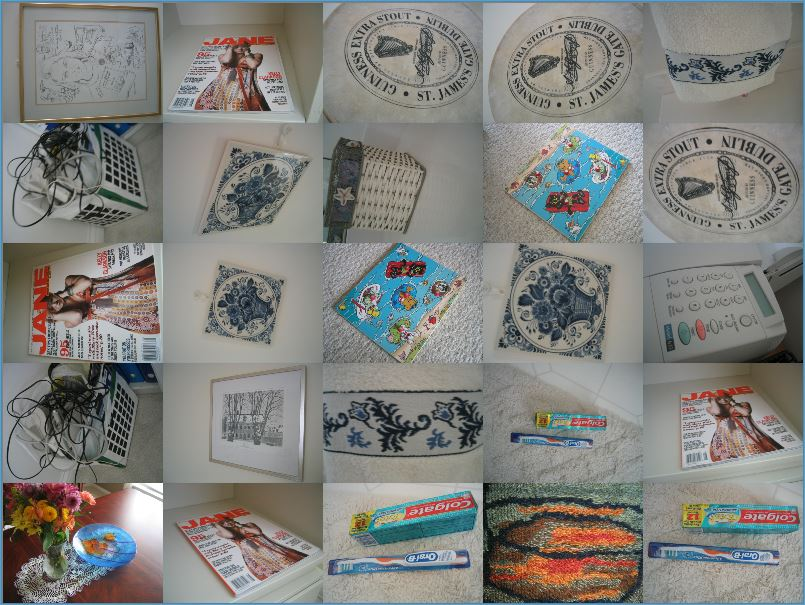
\includegraphics[width=0.49\textwidth]{img/SURF_knn=25_linear.JPG}}
  \caption{Résultats de l'algorithme avec la base de données NISTER}
  \label{db}
\end{figure}

\section{Conclusion}

Notre algorithme permet dans tous les cas testés de retrouver l'image requête. Néanmoins, une très légere variation dans l'image peut influencer 
sa position dans les résultats de façon très importante. 
De plus, selon le cas et le type de résulats souhaités (précis ou larges), on peut adapter le choix du descripteur.
Pour améliorer nos résultats, il faudrait ajouter des traitements en plus sur les images, par exemple de type comparaison d'histogrammes, pour affiner la recherche.
\end{document}

